\section*{Appendix}

\subsection*{A. Additional Figures}

\begin{figure}[h]
\centering
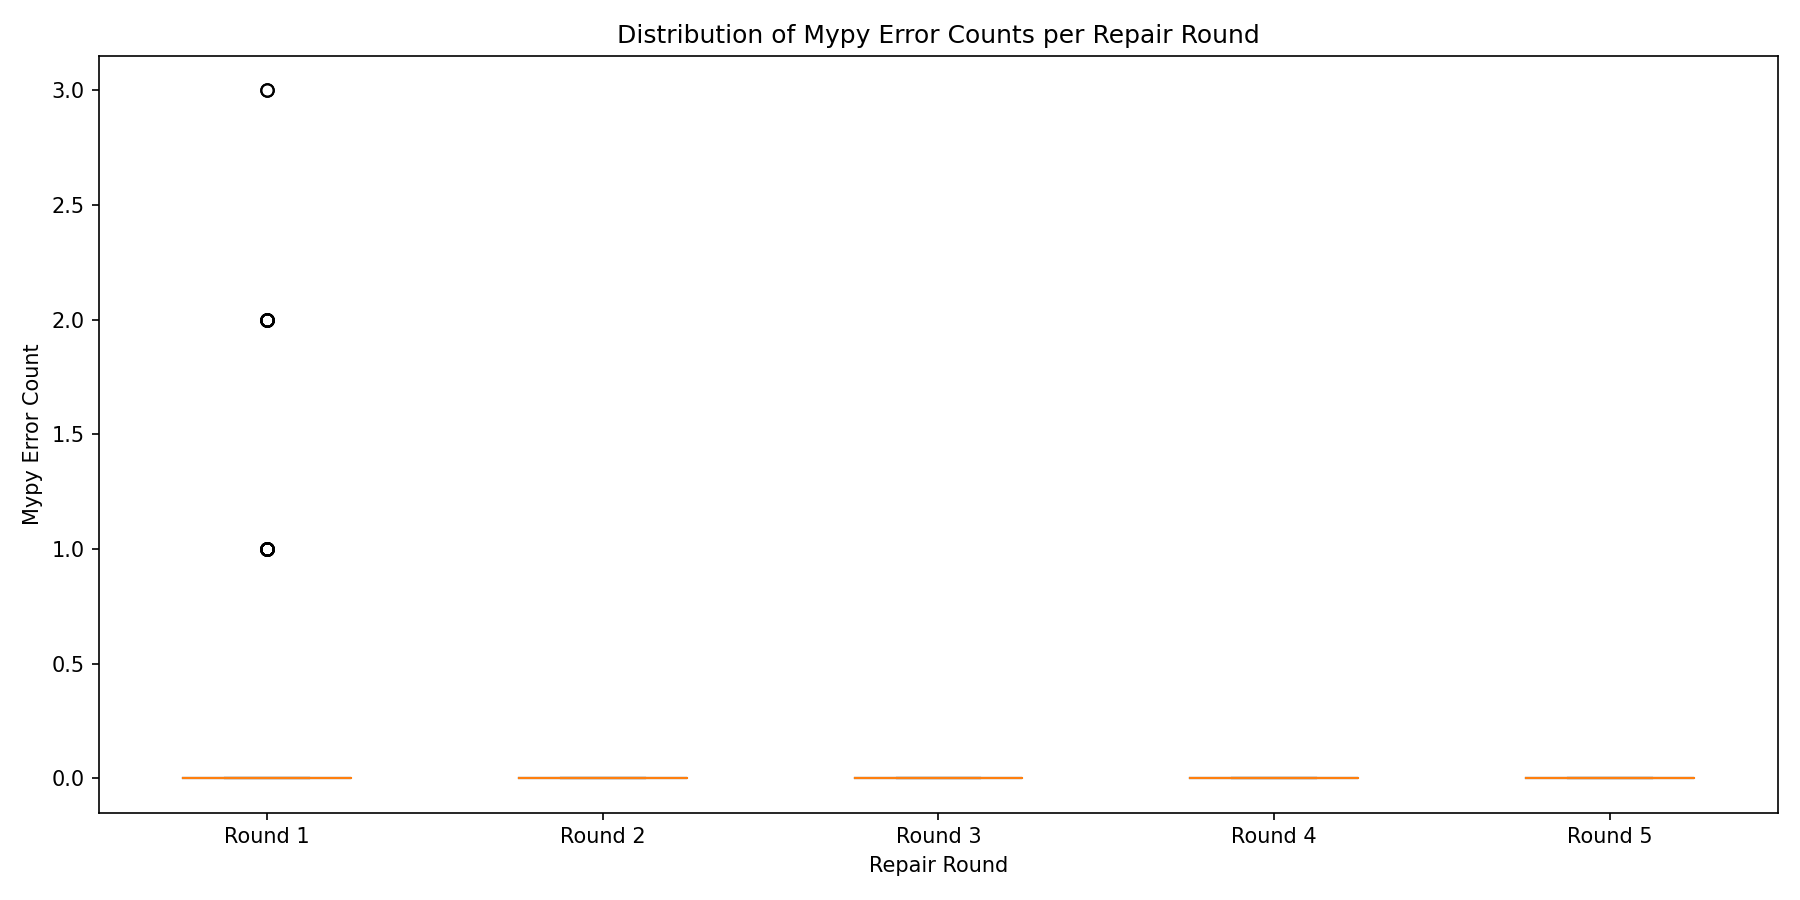
\includegraphics[width=0.9\columnwidth]{figures/error_distribution.png}
\caption{Distribution of mypy error counts across HumanEval+ failing solutions.}
\label{fig:error_distribution}
\end{figure}

\begin{figure}[h]
\centering
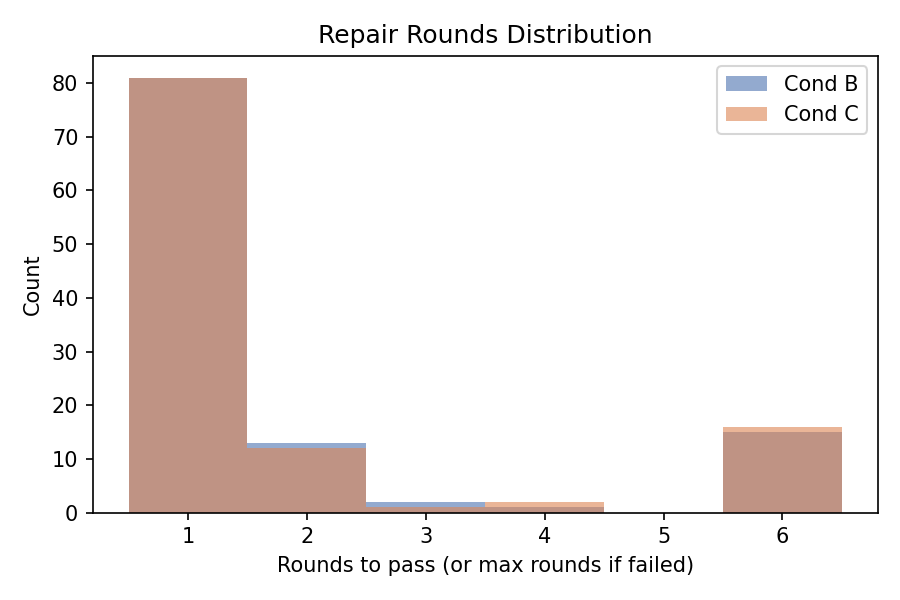
\includegraphics[width=0.9\columnwidth]{figures/repair_rounds.png}
\caption{Pass@1 by repair round for Conditions A and B on HumanEval+.}
\label{fig:repair_rounds}
\end{figure}

\begin{figure}[h]
\centering
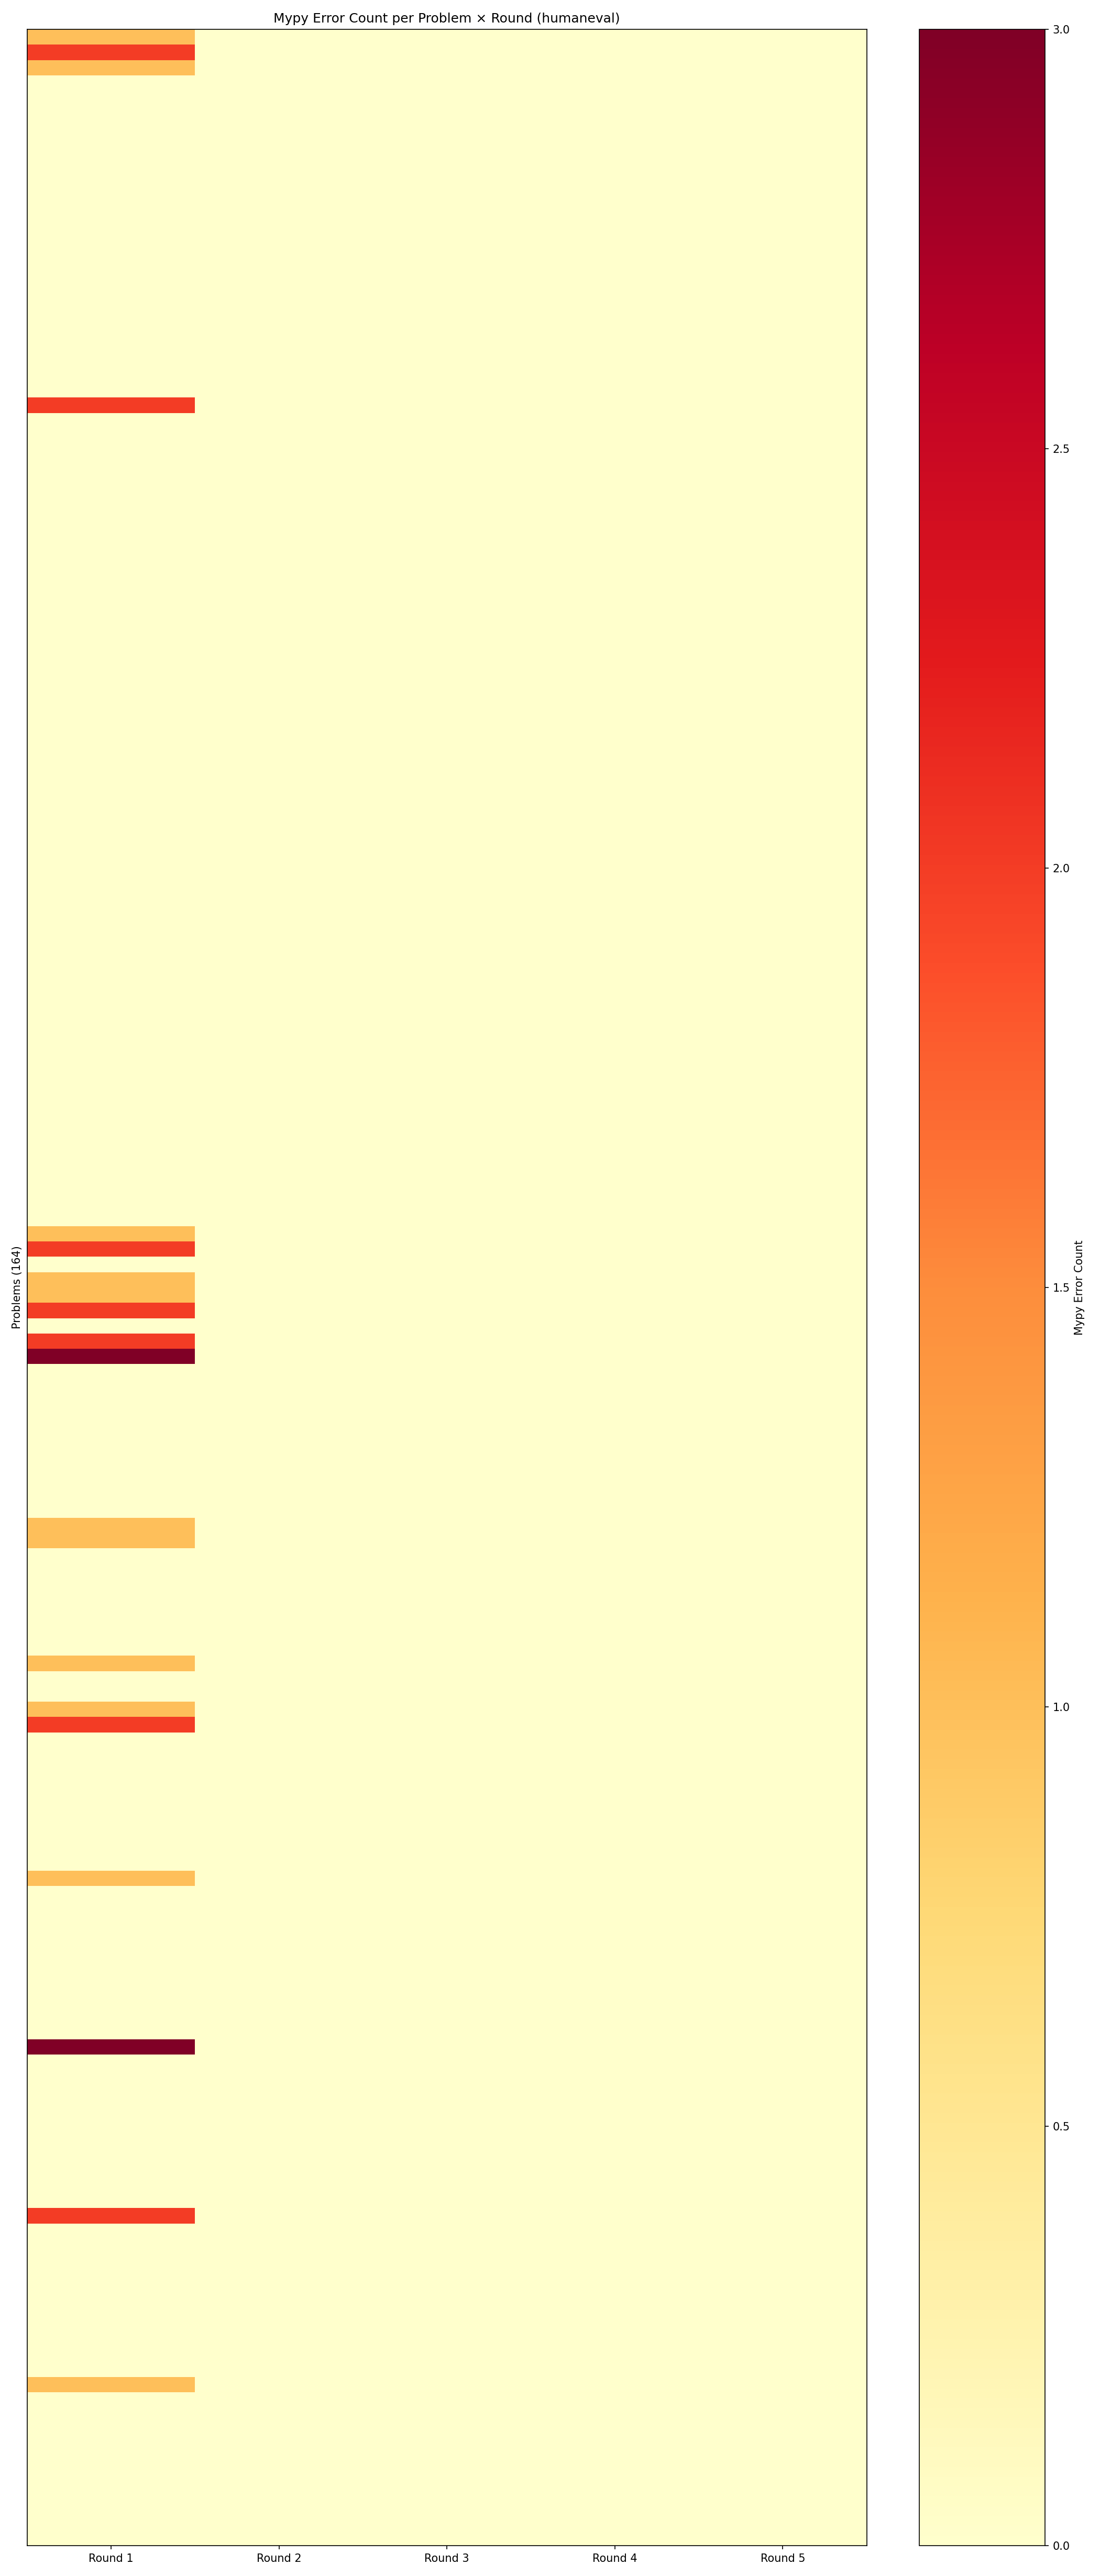
\includegraphics[width=0.9\columnwidth]{figures/heatmap_humaneval.png}
\caption{Per-problem pass/fail heatmap for Conditions A and B across seeds
on HumanEval+.}
\label{fig:heatmap}
\end{figure}

\subsection*{B. Implementation Notes}

All code is implemented in Python 3.10. The repair loop harness makes
sequential API calls to GPT-4o-mini with exponential backoff on rate-limit
errors. mypy is invoked as a subprocess with a 30-second timeout per call.
Z3 (version 4.12) is invoked via the \texttt{z3-solver} Python package.
EvalPlus version 0.2.0 is used for test harness evaluation. All experiments
were run on a single machine with 32GB RAM; wall-clock time for the full
HumanEval+ experiment (3 seeds, 2 conditions) was approximately 6 hours.

\subsection*{C. Prompt Templates}

The repair prompt for Condition B follows this structure:

\begin{verbatim}
System: You are a Python expert. Fix the following code.

Problem: {problem_description}

Current solution:
```python
{current_solution}
```

Execution feedback:
{execution_feedback}

mypy output:
{mypy_output}

Provide the corrected complete Python function.
\end{verbatim}

Condition A omits the ``mypy output'' block. Condition C adds a ``Z3
counterexample'' block after the mypy output block.
